\subsection{前测度的像}

设 E 和 \(E_{1}\) 是局部凸空间，且 u 是从 E 到 \(E_{1}\) 的连续线性映射。对于每个 \(V_{1} \in \mathcal{F}(E_{1})\)，子空间 \(V = \overline{u}^{1}(V_{1})\) 属于 \(\mathcal{F}(E)\)，并且 u 通过取商定义线性映射 \(u_{V_{1}}\)，其从 E/V 到 \(E_{1}/V_{1}\)。设 \(V_{1}\) 和 \(W_{1}\) 是 \(\mathcal{F}(E_{1})\) 中的元素，满足 \(V_{1} \supset W_{1}\)，并置 \(V = \overline{u}^{1}(V_{1})\)，\(W = \overline{u}^{1}(W_{1})\)，则 \(V \supset W\)，并有如下交换图。

\pandocbounded{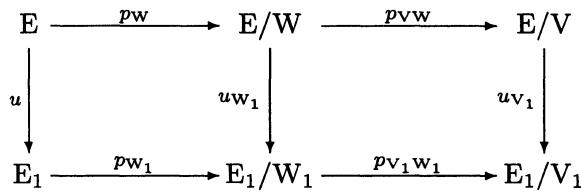
\includegraphics[keepaspectratio]{images/part002_2ec1bcbe.jpg}}

现在设 \(\mu = (\mu_{\mathrm{V}})_{\mathrm{V}\in \mathcal{F}(\mathrm{E})}\) 是 \(\mathbf{E}\) 上的前测度。对每个 \(\mathrm{V}_1\in \mathcal{F}(\mathrm{E}_1)\)，置

\[
\nu_ {\mathrm{V} _ {1}} = u _ {\mathrm{V} _ {1}} \left(\mu_ {u ^ {- 1} \left(\mathrm{V} _ {1}\right)}\right).\tag{1}
\]

前述图的交换性表明，族 \(\nu = (\nu_{\mathrm{V}_1})_{\mathrm{V}_1 \in \mathcal{F}(\mathrm{E}_1)}\) 是 \(\mathbf{E}_1\) 上的前测度。称 \(\nu\) 为 \(\mu\) 在 \(u\) 下的像，并记为 \(u(\mu)\)。

设 \(\lambda\) 是 E 上的有界测度，且 \(u(\lambda)\) 是 \(E_{1}\) 上的测度，是 \(\lambda\) 在 u 下的像。若前测度 \(\mu\) 与 \(\lambda\) 对应，则前测度 \(u(\mu)\) 与 \(u(\lambda)\) 对应。这由前述图的交换性得出。

设 \(V \in \mathcal{F}(E)\)。显然，定义在 \(E/V\) 上的、\(\mu\) 经典范映射 \(p_V: E \to E/V\) 得到的像前测度与测度 \(\mu_V\) 对应。

设 \(u_{1}\) 是从 \(E_{1}\) 到局部凸空间 \(E_{2}\) 的连续线性映射。容易证明关系

\[
(u _ {1} \circ u) (\mu) = u _ {1} (u (\mu))
\]

（前测度像的传递性）。

